\documentclass[11pt]{article}
\usepackage[top=1cm, bottom=2cm, left=1cm, right=1cm]{geometry}
\usepackage{ctex}
\usepackage{algorithm}
\usepackage{algorithmicx}
\usepackage{algpseudocode}
\usepackage{amsthm,amsmath,amssymb}
\usepackage[colorlinks=true,linkcolor=blue]{hyperref}
\usepackage{listings}
\usepackage{xcolor,xparse}
\usepackage{realboxes}
\usepackage{graphics}
\usepackage{graphicx}
\usepackage{mathrsfs}
\usepackage{wrapfig}
\usepackage{subfigure}
\usepackage{pifont}
\newcommand{\To}{\textbf{To} }
\definecolor{cmdbg}{rgb}{0.9,0.9,0.9}
\lstset{%
	basicstyle=\ttfamily,
	breaklines = true,
	backgroundcolor=\color{cmdbg},
}
\DeclareDocumentCommand{\ccmd}{v}{% 参数 v 表示工作方法类似于 \verb
    \Colorbox{cmdbg}{\csname lstinline\endcsname!#1!}%
}

\makeatletter
\newenvironment{breakablealgorithm}
  {% \begin{breakablealgorithm}
   \begin{center}
     \refstepcounter{algorithm}% New algorithm
     \hrule height.8pt depth0pt \kern2pt% \@fs@pre for \@fs@ruled
     \renewcommand{\caption}[2][\relax]{% Make a new \caption
       {\raggedright\textbf{\ALG@name~\thealgorithm} ##2\par}%
       \ifx\relax##1\relax % #1 is \relax
         \addcontentsline{loa}{algorithm}{\protect\numberline{\thealgorithm}##2}%
       \else % #1 is not \relax
         \addcontentsline{loa}{algorithm}{\protect\numberline{\thealgorithm}##1}%
       \fi
       \kern2pt\hrule\kern2pt
     }
  }{% \end{breakablealgorithm}
     \kern2pt\hrule\relax% \@fs@post for \@fs@ruled
   \end{center}
  }
\makeatother

\author{谢昀城 22307110070}
\title{计算物理作业7}

\begin{document}
\maketitle




  \section{题目1}
  \subsection{题目描述}
  
  Write a code to numerically solves the motion of a simple pendulum using Euler’s method, midpoint method, RK4, Euler-trapezoidal method (implement these methods by yourself). Plot the angle and total energy as a function of time. Explain the results.


\subsection{程序描述}
   在本程序中我们将使用Euler’s method, midpoint method, RK4, Euler-trapezoidal method计算单摆的运动,并通过绘制$\theta-t$,$\dot{\theta}-t$,$E-t$图来测试结果的稳定性。

本程序源文件为simplePendulum.py,在终端进入当前目录,使用命令python -u simplePendulum.py运行本程序。运行时请保证Python第三方库Numpy,Matplotlib已安装。程序开发环境为Python3.12.3,可在Python3.8以上版本中运行。

\subsection{伪代码}
\subsubsection*{Pendulum Class:}
\begin{breakablealgorithm}
  \caption{PendulumClass}
  \begin{algorithmic}
  
    \State \textbf{Class:}Pendulum($m, g, \theta, \dot{\theta}$)
    \State \textbf{method:}
    \Function{GetA}{}
      \State \textbf{OUTPUT:} acceleration
      \State \text{acceleration} $\gets -g \times m \times \sin(\theta)$
      \State \Return \text{acceleration}
    \EndFunction
  
    \Function{GetZ}{}
      \State \textbf{OUTPUT:} stateVector
      \State \text{stateVector} $\gets \text{array}([\theta, \dot{\theta}])$
      \State \Return \text{stateVector}
    \EndFunction
  
    \Function{GetHZ}{}
      \State \textbf{OUTPUT:} differentialStateVector
      \State \text{differentialStateVector} $\gets \text{array}([\dot{\theta}, \text{GetA}()])$
      \State \Return \text{differentialStateVector}
    \EndFunction
  
    \Function{Update}{$newtheta, newdtheta$}
      \State \textbf{INPUT:} $newtheta$ (new angle), $newdtheta$ (new angular velocity)
      \State $\theta \gets \text{mod}(newtheta + \pi, 2 \times \pi) - \pi$
      \State $\dot{\theta} \gets dtheta$
    \EndFunction
    \State \textbf{end Class}
  \end{algorithmic}
  \end{breakablealgorithm}
\subsection*{EulerStep:}
  
\begin{breakablealgorithm}
  \caption{EulerStep}
  \begin{algorithmic}
  
    \Function{EulerStep}{$pendulum, dt$}
      \State \textbf{INPUT:} $pendulum$ (Pendulum object), $dt$ (time step)
      \State \textbf{OUTPUT:} None
      \State $z \gets pendulum.\text{GetZ}()$
      \State $Hz \gets pendulum.\text{GetHZ}()$
      \State $z \gets z + Hz \times dt$
      \State $pendulum.\text{Update}(z[0], z[1])$
    \EndFunction
  
  \end{algorithmic}
\end{breakablealgorithm}
\subsection*{MidpointStep:}
\begin{breakablealgorithm}
  \caption{MidpointStep}
  \begin{algorithmic}
  
    \Function{MidpointStep}{$pendulum, dt$}
      \State \textbf{INPUT:} $pendulum$ (Pendulum object), $dt$ (time step)
      \State \textbf{OUTPUT:} None
      \State $z \gets pendulum.\text{GetZ}()$
      \State $Hz \gets pendulum.\text{GetHZ}()$
      \State $z \gets z + Hz \times \frac{dt}{2}$
      \State $pendulum.\text{Update}(z[0], z[1])$
      \State $Hz \gets pendulum.\text{GetHZ}()$
      \State $z \gets z + Hz \times \frac{dt}{2}$
      \State $pendulum.\text{Update}(z[0], z[1])$
    \EndFunction
  
  \end{algorithmic}
  \end{breakablealgorithm}
  
  \subsection*{RK4Step:}
  \begin{breakablealgorithm}
    \caption{RK4Step}
    \begin{algorithmic}
    
      \Function{RK4Step}{$pendulum, dt$}
        \State \textbf{INPUT:} $pendulum$ (Pendulum object), $dt$ (time step)
        \State \textbf{OUTPUT:} None
        \State $z \gets pendulum.\text{GetZ}()$
        \State $Hz \gets pendulum.\text{GetHZ}()$
        \State $k1 \gets Hz \times dt$
        \State $pendulum.\text{Update}(z[0] + \frac{k1[0]}{2}, z[1] + \frac{k1[1]}{2})$
        \State $Hz \gets pendulum.\text{GetHZ}()$
        \State $k2 \gets Hz \times dt$
        \State $pendulum.\text{Update}(z[0] + \frac{k2[0]}{2}, z[1] + \frac{k2[1]}{2})$
        \State $Hz \gets pendulum.\text{GetHZ}()$
        \State $k3 \gets Hz \times dt$
        \State $pendulum.\text{Update}(z[0] + k3[0], z[1] + k3[1])$
        \State $Hz \gets pendulum.\text{GetHZ}()$
        \State $k4 \gets Hz \times dt$
        \State $pendulum.\text{Update}(z[0] + \frac{k1[0] + 2 \times k2[0] + 2 \times k3[0] + k4[0]}{6}, z[1] + \frac{k1[1] + 2 \times k2[1] + 2 \times k3[1] + k4[1]}{6})$
      \EndFunction
    
    \end{algorithmic}
    \end{breakablealgorithm}

    \subsection*{EulerTrapezoidalStep:}
    
    \begin{breakablealgorithm}
      \caption{EulerTrapezoidalStep}
      \begin{algorithmic}
      
        \Function{EulerTrapezoidalStep}{$pendulum, dt, tol = 1e-6, maxiter = 1000$}
          \State \textbf{INPUT:} $pendulum$ (Pendulum object), $dt$ (time step), $tol$ (tolerance), $maxiter$ (maximum iterations)
          \State \textbf{OUTPUT:} None
          \State $z0 \gets pendulum.\text{GetZ}()$
          \State $Hz0 \gets pendulum.\text{GetHZ}()$
          \State $z \gets z0.\text{Copy}()$
          
          \For{$i \gets 0$ \textbf{to} $maxiter - 1$}
            \State $Hzi \gets pendulum.\text{GetHZ}()$
            \State $pendulum.\text{Update}(z0[0] + \frac{Hz0[0] \times dt}{2} + \frac{Hzi[0] \times dt}{2}, z0[1] + \frac{Hz0[1] \times dt}{2} + \frac{Hzi[1] \times dt}{2})$
            \State $zhis \gets z.\text{Copy}()$
            \State $z \gets pendulum.\text{GetZ}()$
            
            \If{$\text{np.linalg.norm}(z - zhis) < tol$}
              \State \textbf{break}
            \EndIf
          \EndFor
        \EndFunction
      
      \end{algorithmic}
      \end{breakablealgorithm}
      
  
  \subsection{输入输出实例}

  对于本程序,运行后会生成图\ref{fig:1}至\ref{fig:6}为"pendulum\_dt=\$dt\_method=\$method.png"至当前目录output路径下,分别为不同求解方法得到的$\theta-t$,$\dot{\theta}-t$,$E-t$图像。程序运行截图为图\ref{fig:7}。

  从图\ref{fig:1}-\ref{fig:4}可以看到在$dt=0.1s$时,在0-100s范围内,Euler方法和Midpoint方法的结果随着时间增长,角度振幅和能量快速发散,且Euler方法增长更大。而RK4和EulerTrapezoidal方法的结果稳定,能量和角度振幅基本保持不变,RK4方法观察到能量随时间轻微减小。

  为放大RK4和EulerTrapezoidal方法的结果的区别,我们将时间范围扩大至1000s,$dt=1.0s$,从\ref{fig:5}-\ref{fig:6}可以看到EulerTrapezoidal方法的结果虽然能量出现了一定程度的振荡,但仍然稳定不会发散。而RK4方法的能量则随着时间逐渐衰减到0。这说明通过精度自适应控制迭代次数的EulerTrapezoidal方法能够更好的保持体系的稳定性。
  \begin{figure}[ht]
    \centering
    \includegraphics[width=1.0\linewidth]{photo/pendulum_dt=0.1_method=Euler.png}
    \caption{Euler method of 0 to 100s,dt=0.1s}
    \label{fig:1}
  \end{figure}

  \begin{figure}[ht]
    \centering
    \includegraphics[width=1.0\linewidth]{photo/pendulum_dt=0.1_method=Midpoint.png}
    \caption{Midpoint method of 0 to 100s,dt=0.1s}
    \label{fig:2}
  \end{figure}

  \begin{figure}
    \centering
    \includegraphics[width=1.0\linewidth]{photo/pendulum_dt=0.1_method=Rk4.png}
    \caption{RK4 method of 0 to 100s,dt=0.1s}
    \label{fig:3}
  \end{figure}

  \begin{figure}
    \centering
    \includegraphics[width=1.0\linewidth]{photo/pendulum_dt=0.1_method=EulerTrapezoidal.png}
    \caption{EulerTrapezoidal method of 0 to 100s,dt=0.1s}
    \label{fig:4}
  \end{figure}

  \begin{figure}
    \centering
    \includegraphics[width=1.0\linewidth]{photo/pendulum_dt=1.0_method=Rk4.png}
    \caption{RK4 method of 0 to 1000s,dt=1.0s}
    \label{fig:5}
  \end{figure}

  \begin{figure}
    \centering
    \includegraphics[width=1.0\linewidth]{photo/pendulum_dt=1.0_method=EulerTrapezoidal.png}
    \caption{EulerTrapezoidal method of 0 to 1000s,dt=0.1s}
    \label{fig:6}
  \end{figure}

  \begin{figure}
    \centering
    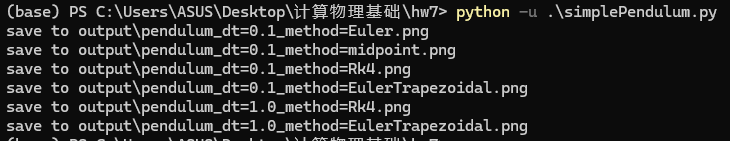
\includegraphics[width=0.8\linewidth]{photo/figp1.png}
    \caption{题目1程序运行截图}
    \label{fig:7}
  \end{figure}
  
\section{题目2}
Write a code to numerically solve the radial Schrödinger equation for
\[
\left[ -\frac{1}{2} \nabla^2 + V(r) \right] \psi(r) = E \psi(r), \quad V(r) = V(r)
\]

For the hydrogen atom:
\[
V(r) = -\frac{1}{r}.
\]

For the local potential:
\[
V_{\text{loc}}(r) = -\frac{Z_{\text{ion}}}{r} \, \text{erf} \left( \frac{r}{\sqrt{2} r_{\text{loc}}} \right)
+ \exp \left[ -\frac{1}{2} \left( \frac{r}{r_{\text{loc}}} \right)^2 \right]
\]

\[
\times \left[ C_1 + C_2 \left( \frac{r}{r_{\text{loc}}} \right)^2
+ C_3 \left( \frac{r}{r_{\text{loc}}} \right)^4
+ C_4 \left( \frac{r}{r_{\text{loc}}} \right)^6 \right].
\]

For the lithium (Li) atom, the constants are:
\[
r_{\text{loc}} = 0.4000000, \quad C_1 = -14.0093922, \quad C_2 = 9.5099073, 
\]
\[
C_3 = -1.7532723, \quad C_4 = 0.0834586, \quad Z_{\text{ion}} = 3.
\]


\subsection{程序描述}
本程序通过有限差分法在均匀和非均匀网格上分别求解H和Li原子的径向薛定谔方程,并比较均匀和非均匀网格的求解效果。

薛定谔方程解可分离变量为$\Psi(r)=R(r)Y_l^m$,$Y_l^m$为球谐函数。径向部分$R(r)$满足方程:
\[
\frac{d}{dr} \left( r^2 \frac{dR}{dr} \right) - 2r^2 \left[ V(r) - E \right] R = l(l+1) R.
\]

令$u(r) = R(r)/r$,则方程可化为:
\[
-\frac{1}{2}\frac{d^2 u}{dr^2} + \left[ V + \frac{l(l+1)}{2 r^2} \right] u = E u.
\]
只需求解u即可。

使用有限差分法,考虑$\frac{d^2u}{dr^2}=\frac{u_{i+1}-u_i-u_{i-1}}{ \Delta r^2}$,和$u_0=u_n=0$边界条件,可将其转换为$Hu=Eu$的矩阵本征值问题。其本征值从小到大依次对应角量子数$l$,主量子数$l+1,l+2,...$的能级。

当采用非均匀网格
\[
r_j = r_p \left[\exp(j\delta) - 1\right], \quad j = 0, 1, \ldots, j_{\text{max}}
\]
\[
r_p = \frac{r_{\text{max}}}{\exp(\delta j_{\text{max}}) - 1}
\]
时,做变换$u_j=u(r_j)=v(j)e^(\delta j/2)$方程将变为(注意:PPT上的$\frac{1}{2 r_p^2\delta^2 e^{2j\delta}}$系数有误)
\[
\frac{1}{2 r_p^2\delta^2 e^{2j\delta}}(-\frac{d^2}{dj^2}v(j)+\delta^2 v(j))+V_eff(j)=-E v(j)
\]
\[
V_eff(j)=V(r_j)+\frac{l(l+1)}{2 r_j^2}
\]
同样可以化为矩阵本征值问题求解。本程序中使用numpy.linalg.eig求解矩阵本征值问题。




程序源文件为solveSchrodinger.py,在终端进入当前目录,使用命令python -u solveSchrodinger.py运行本程序。运行时请保证Python第三方库Numpy,Matplotlib已安装。程序开发环境为Python3.12.3,可在Python3.8以上版本中运行。

\section{伪代码}
\subsection*{均匀网格求解}
\begin{breakablealgorithm}
  \caption{SolveSchrodinger}
  \begin{algorithmic}
  
    \Function{SolveSchrodinger}{$l, n = 1000, rmin = 0, rmax = 100, type = "Li"$}
      \State \textbf{INPUT:} $l$ (angular momentum quantum number), $n$ (number of points), $rmin$ (minimum radius), $rmax$ (maximum radius), $type$ (type of atom)
      \State \textbf{OUTPUT:} $El$ (eigenvalues), $r$ (radius array), $vl$ (eigenvectors)
      
      \State $H \gets$ zero matrix of size $(n, n)$
      \State $dr \gets \frac{rmax - rmin}{n}$
      \State $r \gets \text{linspace}(dr, rmax, n, \text{endpoint} = \text{False})$
      
      \For{$i \gets 0$ \To $n - 1$}
        \State $H[i, i] \gets 1 + \text{Veff}(r[i], l, type) \times dr^2$
        \If{$i < n - 1$}
          \State $H[i, i + 1] \gets -\frac{1}{2}$
          \State $H[i + 1, i] \gets -\frac{1}{2}$
        \EndIf
      \EndFor
      
      \State $re \gets \text{linalg.eigh}(H)$
      \State $El \gets re[0] / dr^2$
      \State $sortedIndices \gets \text{argsort}(El)$
      \State $El \gets El[sortedIndices]$
      \State $vl \gets (re[1])[:, sortedIndices]$
      
      \State \Return $El, r, vl$
    \EndFunction
  
  \end{algorithmic}
  \end{breakablealgorithm}

  \subsection*{非均匀网格求解}
  \begin{breakablealgorithm}
    \caption{SolveSchrodingerNonuniform}
    \begin{algorithmic}
    
      \Function{SolveSchrodingerNonuniform}{$l, jmax = 1000, rmin = 0, rmax = 100, delta = 0.01, type = "Li"$}
        \State \textbf{INPUT:} $l$ (angular momentum quantum number), $jmax$ (number of points), $rmax$ (maximum radius), $delta$ (scaling factor), $type$ (type of atom)
        \State \textbf{OUTPUT:} $El$ (eigenvalues), $r$ (radius array), $vl$ (eigenvectors)
        
        \State $H \gets$ zero matrix of size $(jmax - 1, jmax - 1)$
        \State $rp \gets \frac{rmax}{\exp(delta \times jmax) - 1}$
        
        \Function{a}{$j$}
          \State \Return $2 rp^2 delta^2  \exp(2 j  delta)$
        \EndFunction
        
        \For{$j \gets 1$ \To $jmax - 1$}
          \State $rj \gets rp  (\exp(delta  j) - 1)$
          \State $H[j - 1, j - 1] \gets \frac{2 + delta^2 / 4}{a(j)} + \text{Veff}(rj, l, type)$
          \If{$j < jmax - 1$}
            \State $H[j - 1, j] \gets -\frac{1}{a(j)}$
            \State $H[j, j - 1] \gets -\frac{1}{a(j + 1)}$
          \EndIf
        \EndFor
        
        \State $re \gets \text{linalg.eig}(H)$
        \State $El \gets re[0]$
        \State $sortedIndices \gets \text{argsort}(El)$
        \State $El \gets El[sortedIndices]$
        \State $s \gets (\exp(delta \times \text{arange}(1, jmax) / 2)).\text{reshape}(-1, 1)$
        \State $vl \gets (re[1])[:, sortedIndices] \times s$
        \State $r \gets \text{array}([rp  (\exp(delta  j) - 1) \text{ for } j \text{ in range}(1, jmax)])$
        
        \State \Return $El, r, vl$
      \EndFunction
    
    \end{algorithmic}
    \end{breakablealgorithm}
    
\section{输入输出实例}
运行本程序后,将在控制台输出由1000个格点采用均匀和非均匀网格求解的H和Li的最低的三个能级能量(其中H存在简并)。并生成由非均匀网格求解的H和Li的$n=1,2,3,4$不同$l$的$u(r)=rR(r)$的图像如图\ref{fig:wavefunctionsH}和\ref{fig:wavefunctionsLi},为"wavefunctionsH.png"和"wavefunctionsLi.png"于当前路径下。此外还将输出Li的势能曲线和网格间距变化图(图\ref{fig:potentialLi},\ref{fig:ununiformgrid})为"potentialLi.png"和"ununiformgrid.png"于当前路径下。
最后,我们比较了$n=2,l=1$能级非均匀网格和均匀网格的收敛速率,如图\ref{fig:compare},输出为"compare.png"于当前路径下。为保持格点间距变化速度一致,采用$\delta=5/jmax$
可以看到相同格点数量下,非均匀网格求解的收敛速率和精度都要高于均匀网格,但是非均匀网格的H矩阵是非对称的,也将有更高的计算成本。

最终得到H前三个能级为:
\[E_1=13.6057eV ,n=1,l=0
\]
\[
E_2=-3.4014eV ,n=2,l=0;n=2,l=1
\]
\[
E_3=-1.5117eV ,n=3,l=0;n=3,l=1;n=3,l=2
\]
Li前三个能级为:
\[
E_1=-121.3165eV ,n=1,l=0
\]
\[
E_2=-30.5389eV ,n=2,l=1
\]
\[
E_3=-30.3529eV ,n=2,l=0
\]

程序运行截图如图\ref{fig:p2}。

\begin{figure}
  \centering
  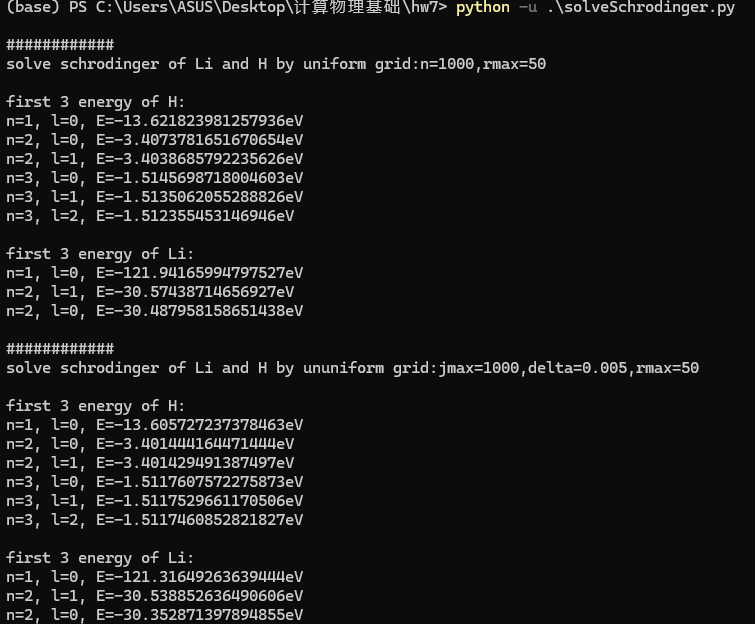
\includegraphics[width=0.8\linewidth]{photo/figp2.png}
  \caption{题目2程序运行截图}
  \label{fig:p2}
\end{figure}


\begin{figure}
  \centering
  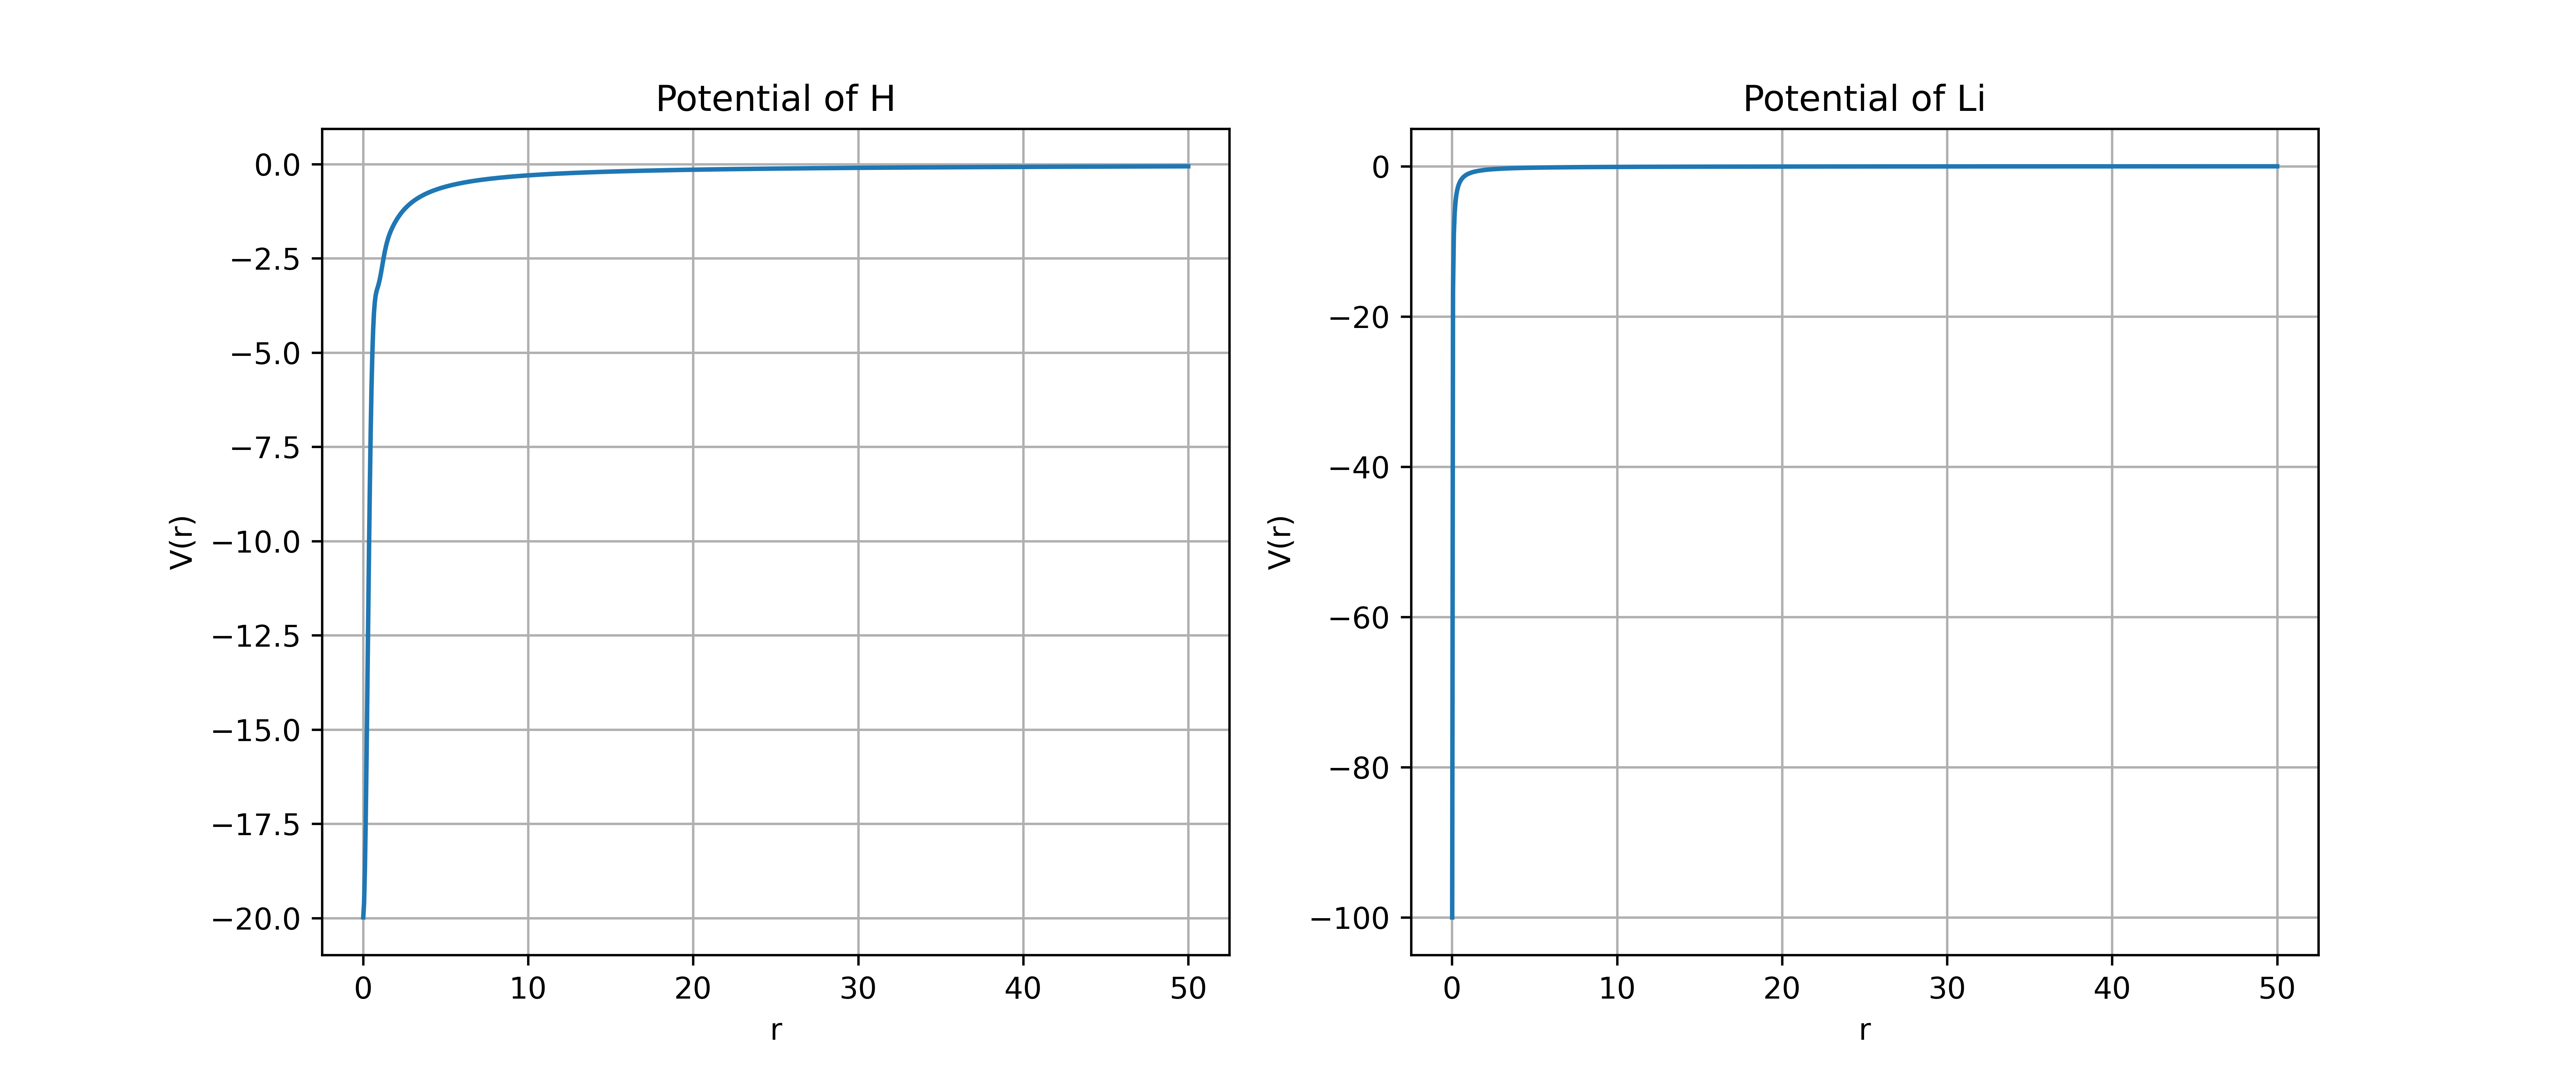
\includegraphics[width=1\linewidth]{photo/potentialLi.png}
  \caption{H和Li原子势能曲线}
  \label{fig:potentialLi}
\end{figure}

\begin{figure}
  \centering
  \includegraphics[width=1\linewidth]{photo/wavefunctionsH.png}
  \caption{H原子不同能级波函数(已归一化)}
  \label{fig:wavefunctionsH}
\end{figure}

\begin{figure}
  \centering
  \includegraphics[width=1\linewidth]{photo/wavefunctionsLi.png}
  \caption{Li原子不同能级波函数(已归一化)}
  \label{fig:wavefunctionsLi}
\end{figure}

\begin{figure}
  \centering
  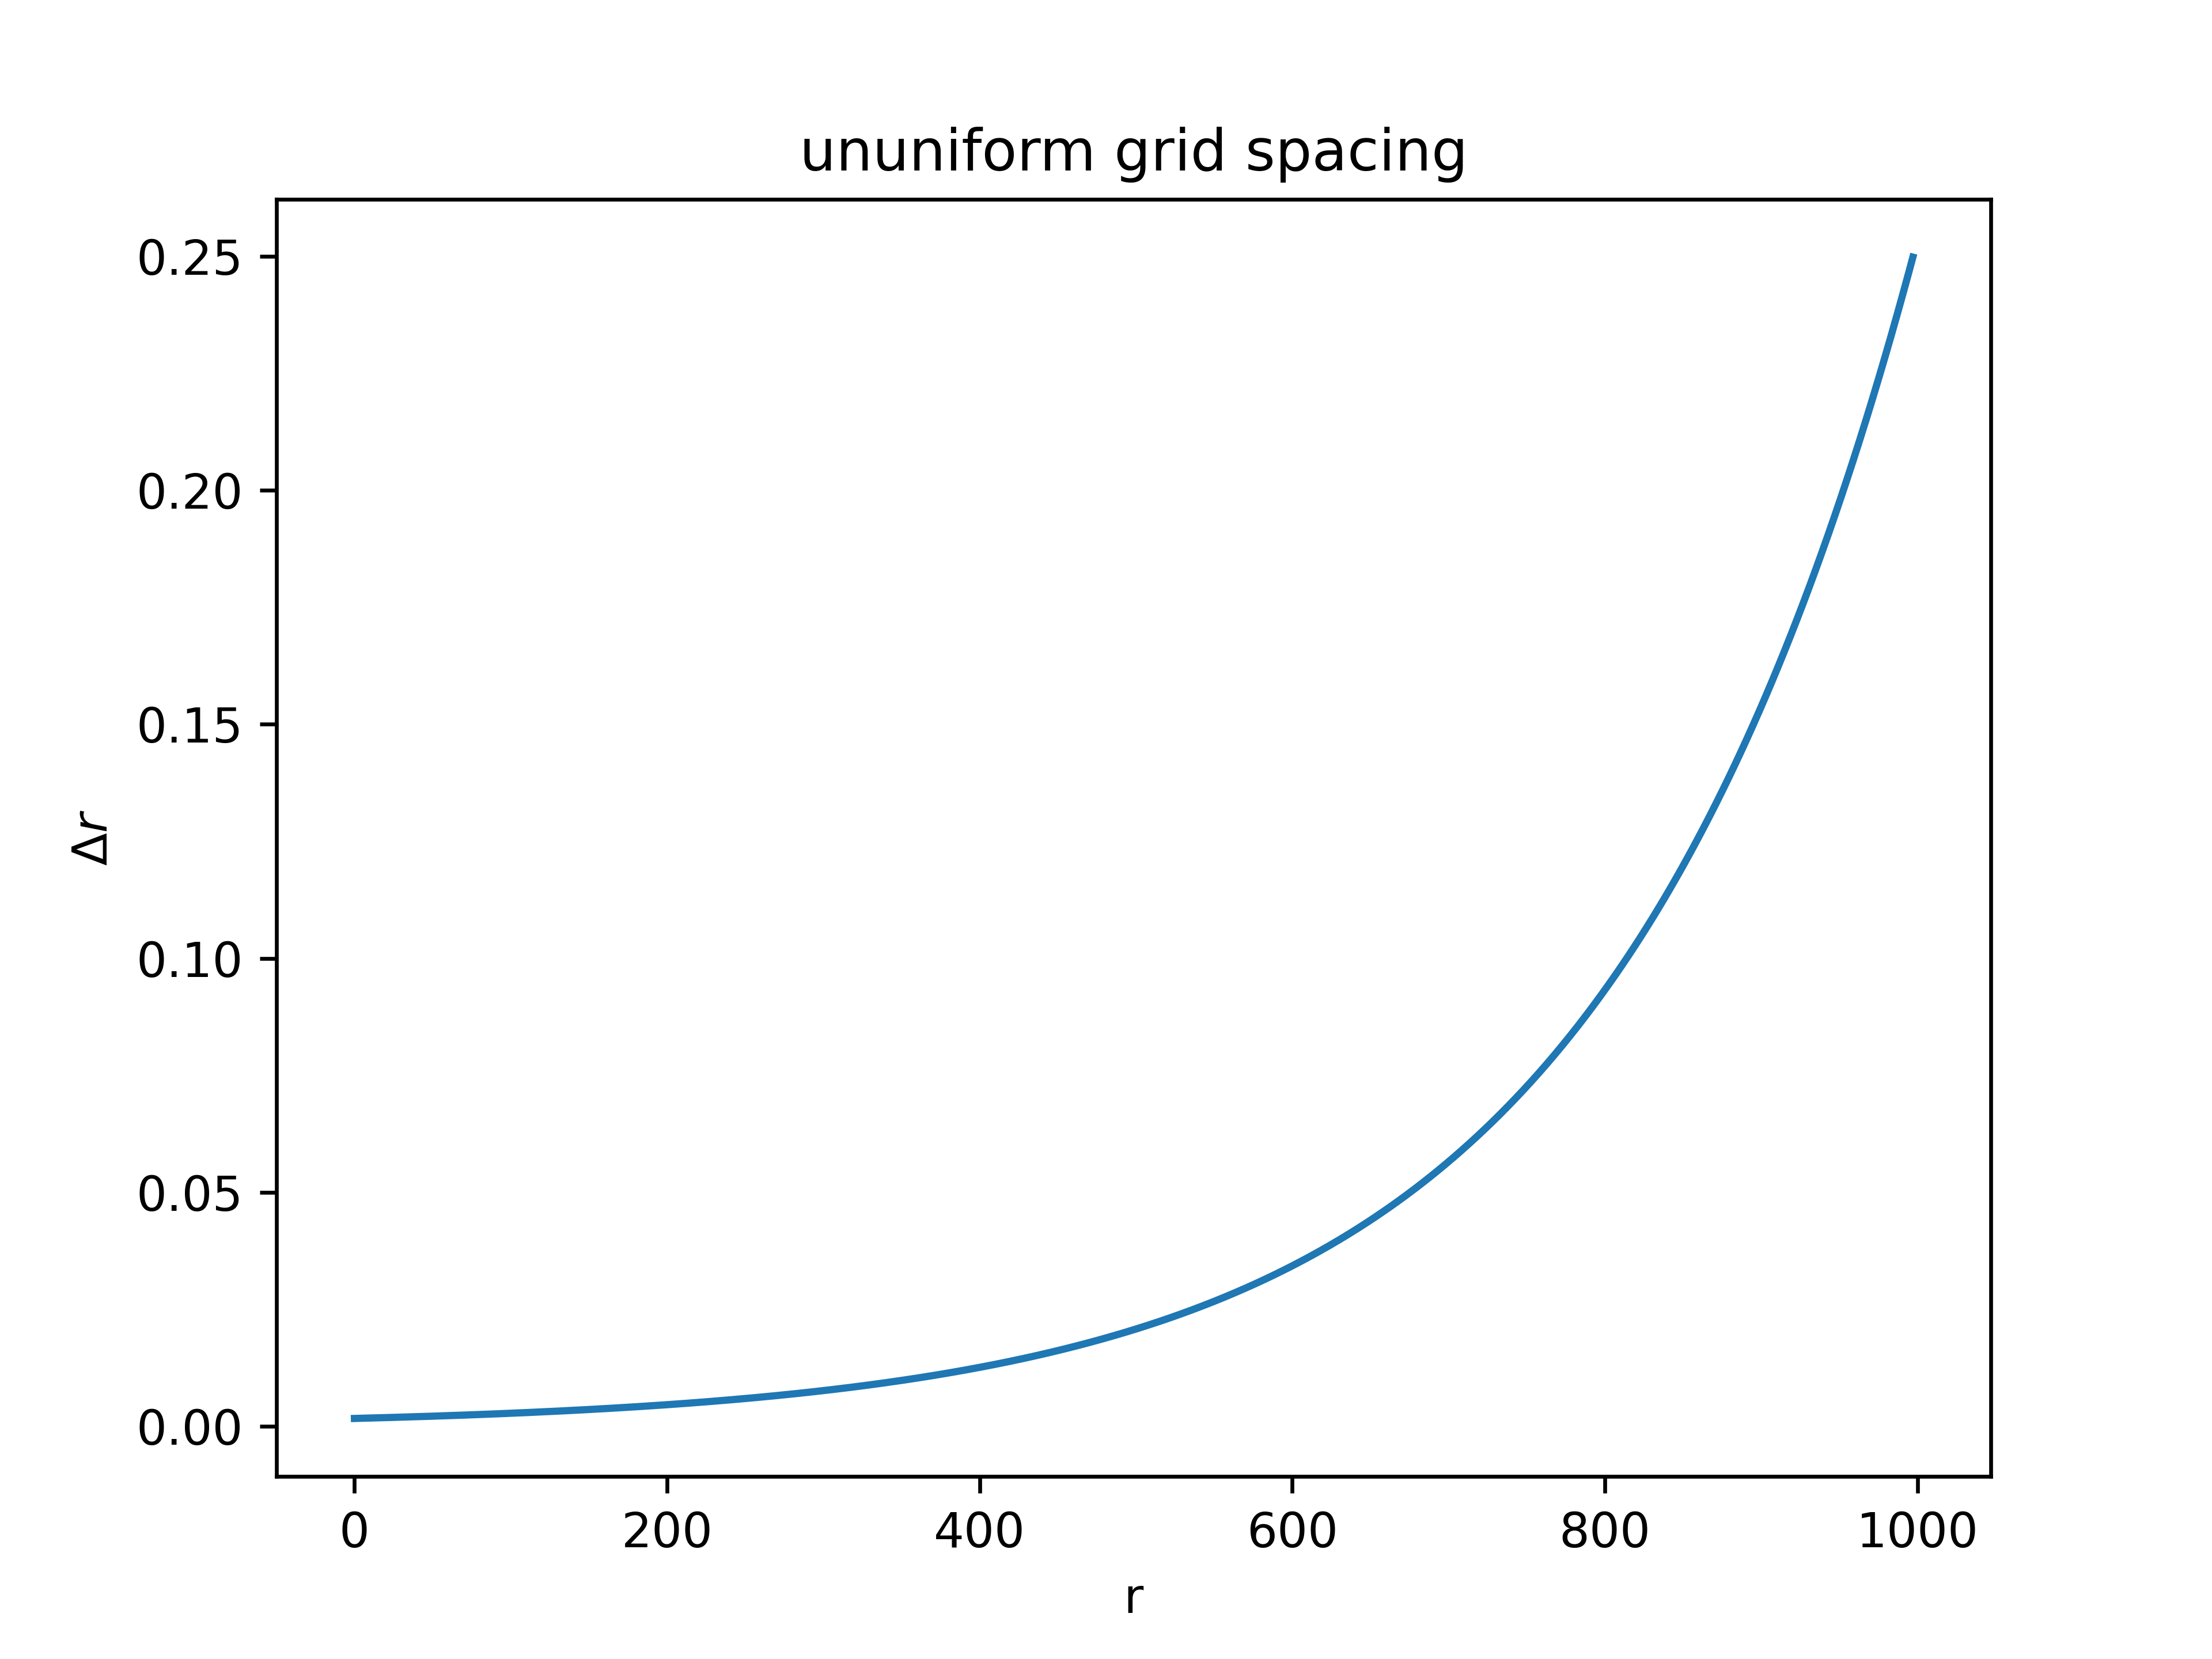
\includegraphics[width=0.8\linewidth]{photo/ununiformgrid.png}
  \caption{非均匀网格间距变化}
  \label{fig:ununiformgrid}
\end{figure}

\begin{figure}
  \centering
  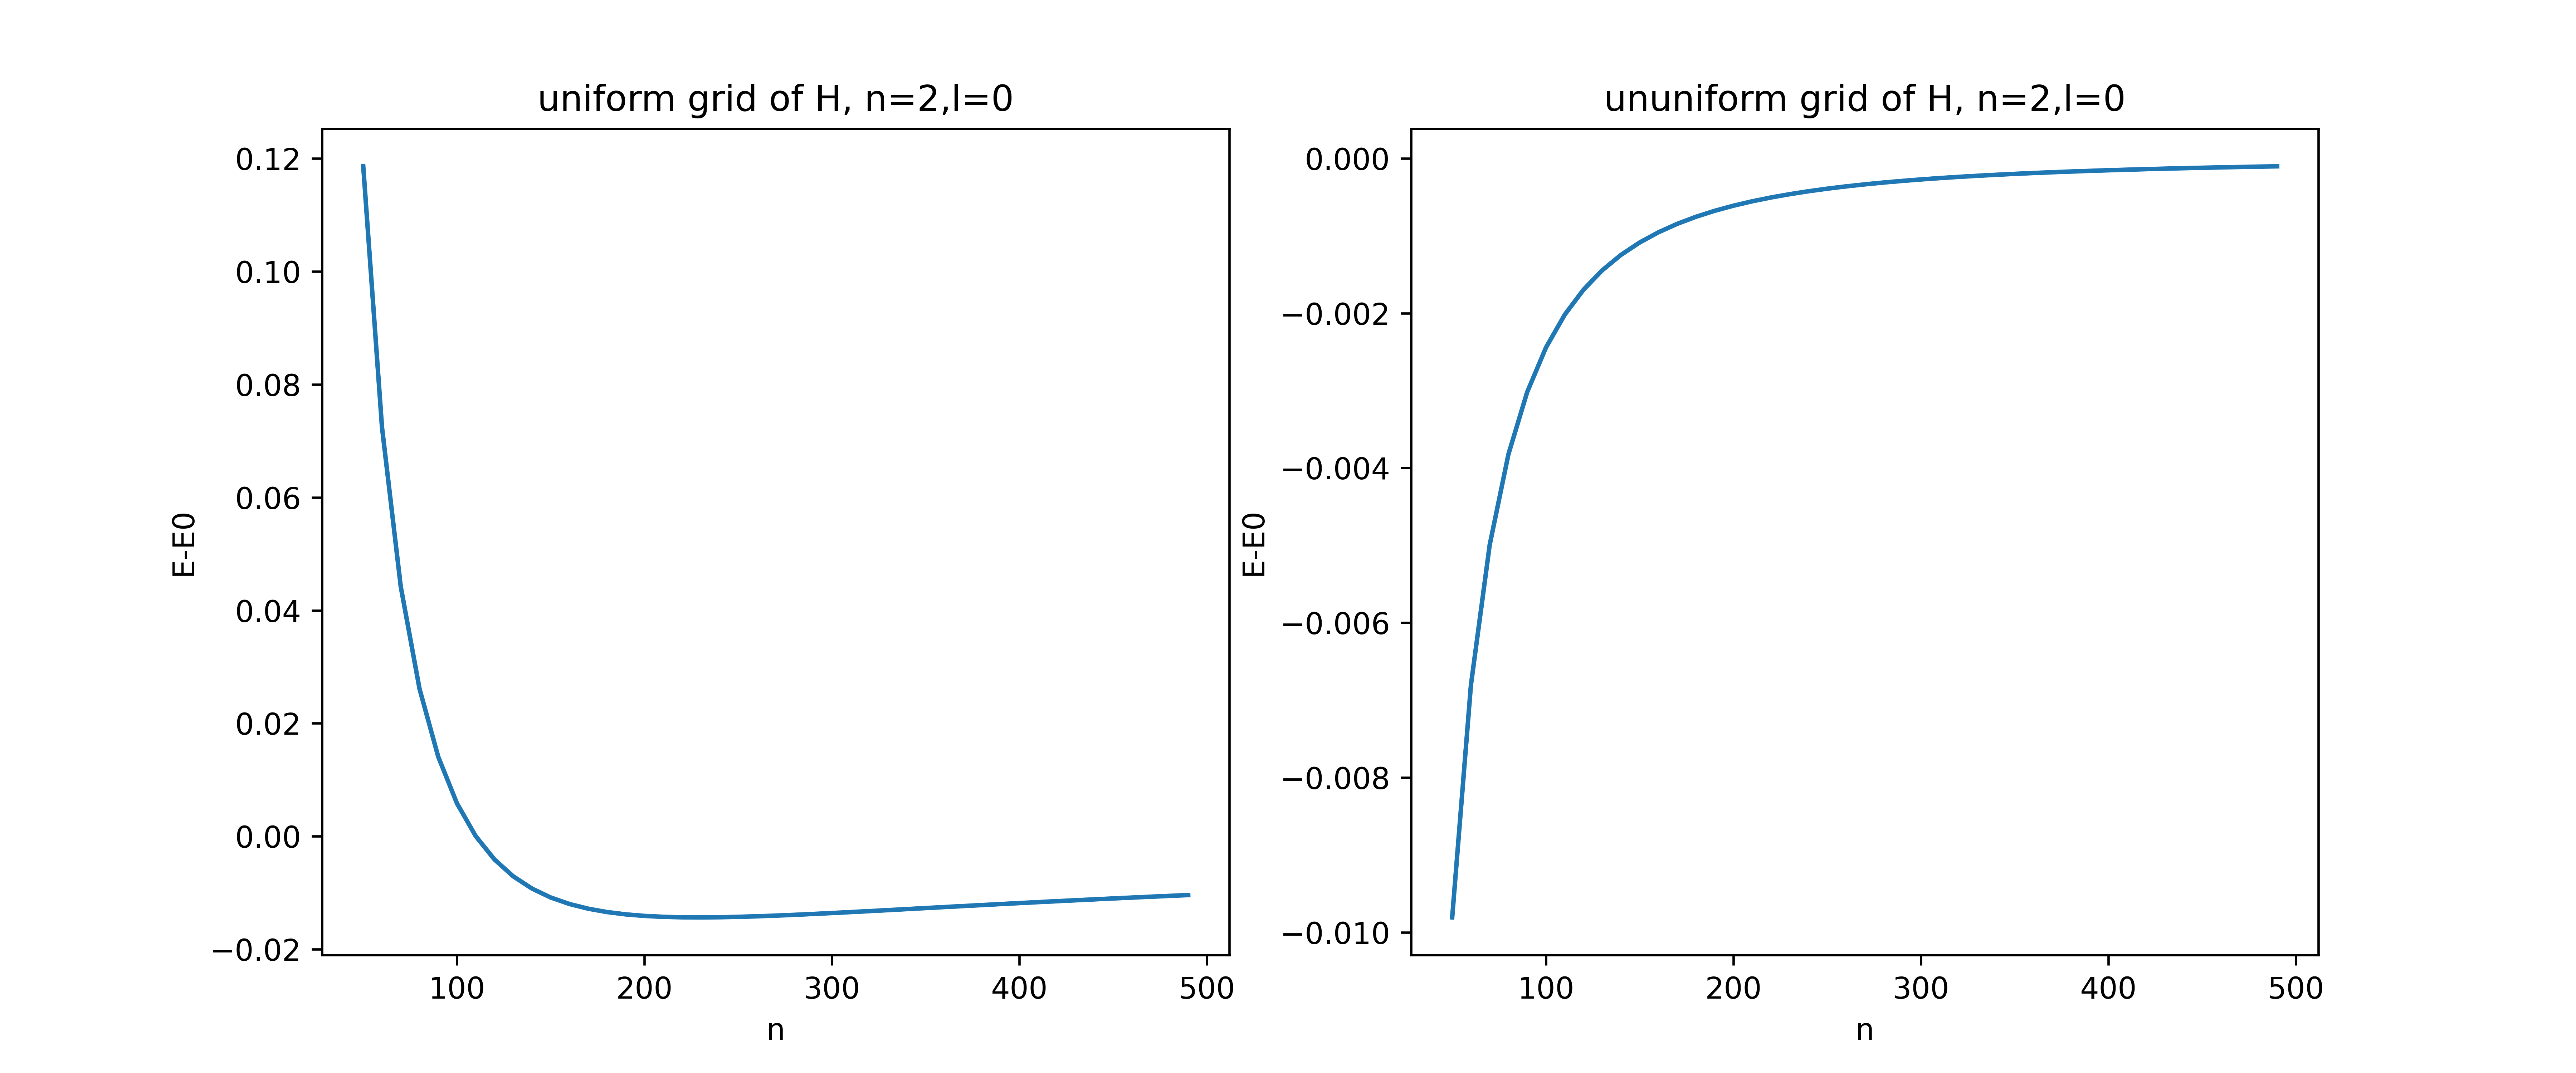
\includegraphics[width=0.8\linewidth]{photo/compare.png}
  \caption{均匀网格和非均匀网格收敛速率比较}
  \label{fig:compare}
\end{figure}


\end{document}


